\documentclass[11pt]{scrartcl}
\usepackage{graphicx}
\graphicspath{{./}}
\usepackage[sexy]{evan}
\usepackage[normalem]{ulem}
\usepackage{hyperref}
\usepackage{mathtools}
\hypersetup{
    colorlinks=true,
    linkcolor=blue,
    filecolor=magenta,      
    urlcolor=cyan,
    pdfpagemode=FullScreen,
    }
\usepackage[most]{tcolorbox}
\renewcommand{\dangle}{\measuredangle}

\renewcommand{\baselinestretch}{1.5}

\addtolength{\oddsidemargin}{-0.4in}
\addtolength{\evensidemargin}{-0.4in}
\addtolength{\textwidth}{0.8in}
% \addtolength{\topmargin}{-0.2in}
% \addtolength{\textheight}{1in} 


\setlength{\parindent}{0pt}

\usepackage{pgfplots}
\pgfplotsset{compat=1.15}
\usepackage{mathrsfs}
\usetikzlibrary{arrows}

\title{Miscellaneous Problems}
\author{Azzam Labib (IG: haxuv.world)}
\date{G3-4 | 2 May 2024}
\begin{document}
\maketitle

\begin{enumerate}
    \section{Logical Thinking and Combinatorics}
    \item Find the 21$^{st}$ term of the arithmetic sequence 27, 35, 43, 51, \ldots


    \vspace{5cm}\item Each of the numbers from 1 to 10 are filled in the circles in the figure so that the sum of each side of the pentagon is 14. What number should be filled in the circle with an A?
    \begin{figure}[h]
        \centering
        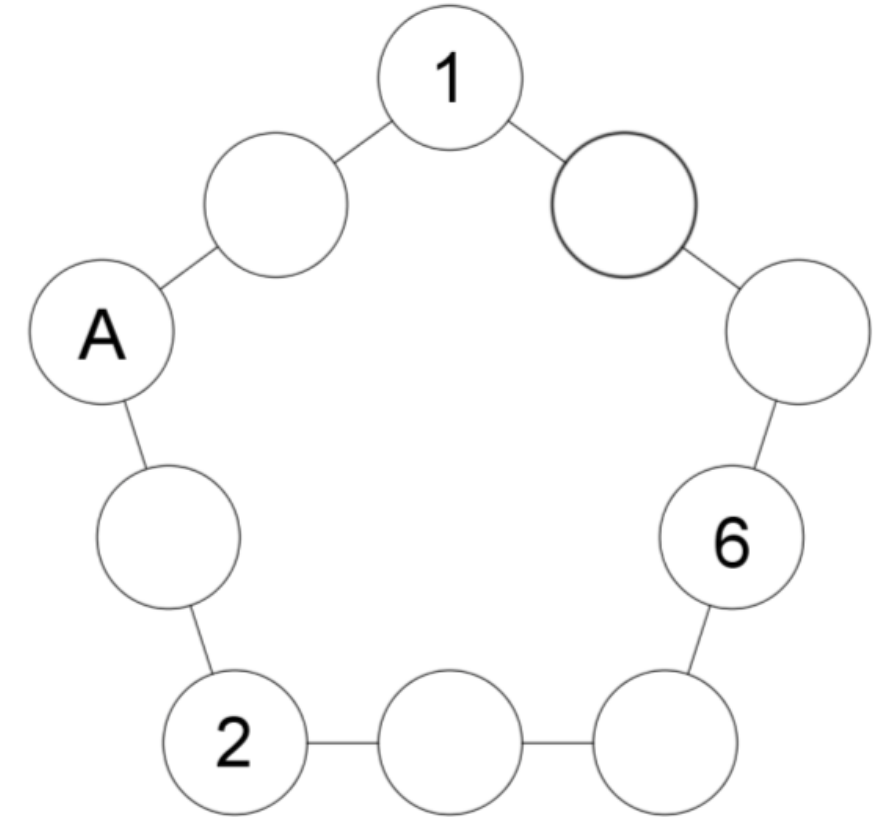
\includegraphics[width=0.4\textwidth]{StarGen/AIMO Trial G3-4 2024/necklace5.png}
    \end{figure}

    \vspace{10cm}\item 10 people takes 5 days to complete one-fourth of a task. How many days are needed for 8 people to finish the same task?

    \vspace{10cm}\item There are 7 pairs of green socks, 6 pairs of white socks, 5 pairs of red socks and 2 pairs of blue socks in a wardrobe. One person is asked to close his eyes, and draw the socks 1 pair at a time. At least how many pairs of socks should be drawn so that among the drawn socks 4 pairs of those have the same colour?
    
    \vspace{10cm}\item Numbers are drawn from the 60 integers 1 to 60. At least how many numbers are drawn at random to ensure that there are two numbers whose difference is 10?

    \vspace{10cm}\item From 1 to 100 (including 1 and 100), at least how many numbers are drawn randomly to ensure that there are two numbers which have 2 or more common factors?
    
    \vspace{13cm}\item 313 boy scouts are divided into groups and each group has at most 7 scouts. At least how many groups can be divided this way?

    \vspace{10cm}
    \section{Arithmetic/Algebra}
    \item Find the value of $12 \times 22 + 13 \times 24 + 17 \times 36$.
    \vspace{10cm}\item Find the value of $480 \div 4 + 480 \div 6 + 480 \div 10$.
    
    \vspace{10cm}\item The amount of Amy's pocket money each day is 3 times as much as the pocket money of Flora's. And the amount of Pearl's pocket money is \$7 more than Amy's. If they have \$980 of pocket money each week, how much pocket money does Pearl have each day?
    
    
    \newpage\item There are a total of 30 chickens and rabbits in a farm. The animals have a total of 86 legs. What is the difference between the number the chickens and the rabbits?

    \vspace{10cm}\item There are some chicken and rabbits. The animals have 304 legs in total. If we count the number of legs using the number of chicken as the number of rabbit, and using the number of rabbit as the number of chicken, there are 338 legs instead. How many chickens are there?

    \vspace{10cm}\item Charles has \$40 in the bank at the beginning. Starting from 1$^{st}$ February, Charles' mother will give Charles pocket money equal to the amount of money in the bank, and Charles saves \$5 every day in the bank. Until the night of the 16$^{th}$ of February, how much (in \$) did Charles' mother gave Charles?

    \vspace{10cm}\item The difference between A and B is 24. A is 9 times of B. Find the value of A.

    
    \vspace{10cm}\item What is the value of $2 + 4 + 6 + \ldots + 100$ ?

    \vspace{10cm}
    \section{Number Theory}
    \item Let $p$ and $q$ be the prime numbers. If $p+q=39$, what is the value of $p \times q$ ?
    
    \vspace{10cm}\item If a 5-digit number $\overline{8175A}$ is divisible by 11, find the value of A.

    \vspace{10cm}\item When a five-digit number $\overline{279A5}$ is divided by 9, the remainder is 4. Find the value of $A$.

    
    \newpage\item A 200-digit number is in the form of '393939\ldots'. The product of digits of the number is calculated, find the unit digit of the product.

    \vspace{10cm}\item If $\overline{ABCD}$ is a 4-digit number divisible by 8 and both $\overline{ABC}$ and $\overline{DCB}$ are divisible by 8. Find the smallest possible value of $\overline{ABCD}$.

    \newpage\item When a five-digit number is divided by 33, the remainder is 11. Find the largest possible value of the number.

    \newpage
    \section{Geometry}
    \item Find the perimeter of the figure below (in cm).
    \begin{figure}[h]
        \centering
        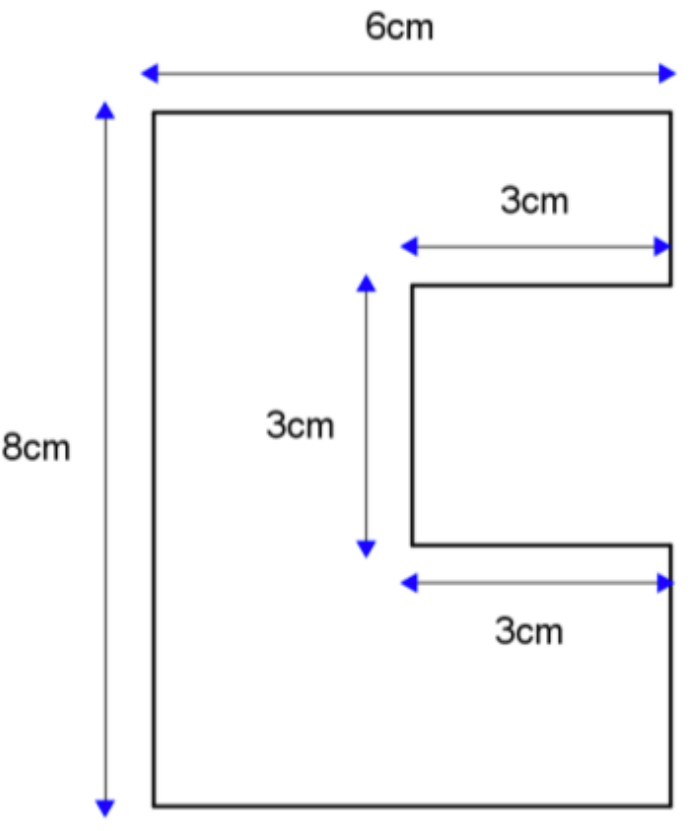
\includegraphics[width=0.43\textwidth]{StarGen/AIMO Trial G3-4 2024/perimeterC.png}
    \end{figure}

    \newpage\item The figure is formed by 2 squares. Find the area of the shaded region (Hint: Consider the relationship between the area of triangle and the area of rectangle)
    \begin{figure}[h]
        \centering
        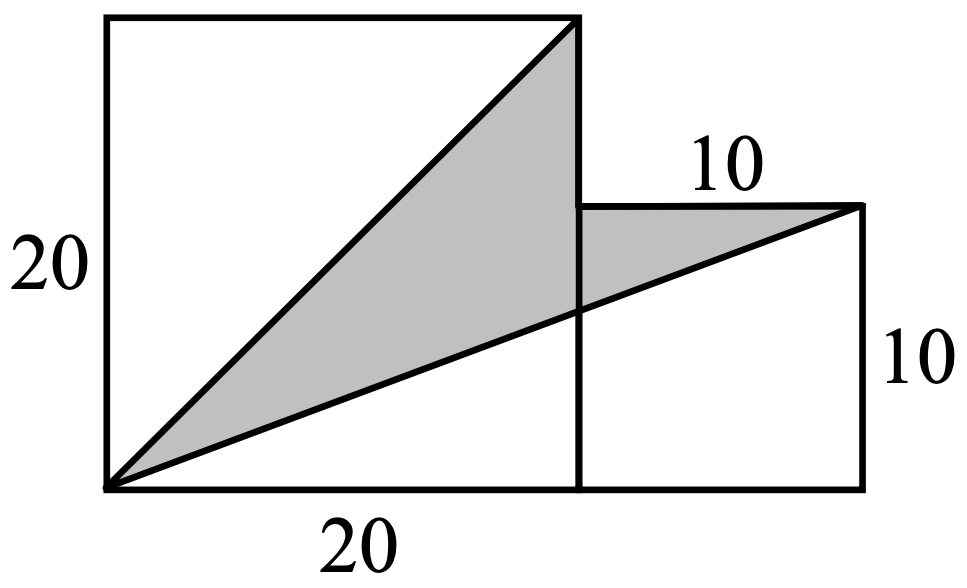
\includegraphics[width=0.4\textwidth]{StarGen/AIMO Trial G3-4 2024/area2sq.png}
    \end{figure}

    \newpage\item The figure shows a figure formed by three identical rectangles and a regular hexagon, if the perimeter of each rectangle is 12 centimetres, what is the perimeter of the figure in centimetres?
    \begin{figure}[h]
        \centering
        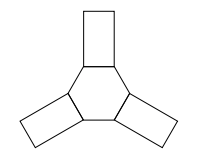
\includegraphics[width=0.4\textwidth]{StarGen/AIMO Trial G3-4 2024/baling2.png}
    \end{figure}

    \newpage\item In the figure, $ABCD$ is a rectangle. The lengths of AE, $EF, FG, GH, HI, IJ$ and $JC$ are 20, 22, 24, 26, 28, 30 and 32 centimetres respectively. What is the difference between the areas of octagon $AEFGHIJD$ and $BEFGHIJC$ in square centimetres?
    \begin{figure}[h]
        \centering
        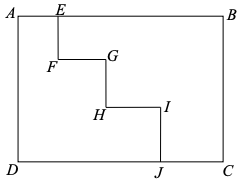
\includegraphics[width=0.4\textwidth]{StarGen/AIMO Trial G3-4 2024/octagon.png}
    \end{figure}
\end{enumerate}

\end{document}